\RequirePackage[l2tabu, orthodox]{nag}

%\documentclass[]{article}
\documentclass[11pt]{scrartcl}
\usepackage[usename, dvipsnames]{xcolor}
\usepackage[pdfencoding=auto]{hyperref}
\usepackage[msc-links]{amsrefs}
\usepackage{cleveref} % use \cref{}, automatically deduces theorem, proposition, etc
\usepackage[mathletters]{ucs}
\usepackage[utf8]{inputenc}
\usepackage[T1]{fontenc}
\usepackage{datetime}

\usepackage{array}
\usepackage{mathtools}
\usepackage{amsmath, amsthm, amssymb, amsfonts, amsxtra, amscd, thmtools}
\let\proof\relax
\let\endproof\relax

% Boxes around theorem environments.
\usepackage[many]{tcolorbox}

\usepackage{color}
%\usepackage{unicode-math}
\usepackage{newunicodechar}
\newunicodechar{ε}{\varepsilon}
\newunicodechar{δ}{\delta}
\newunicodechar{µ}{\mu}
\newunicodechar{→}{\to}
\newunicodechar{≤}{\leq}
\newunicodechar{∈}{\in}
\newunicodechar{⊆}{\subseteq}
\newunicodechar{Λ}{\Lambda}
\newunicodechar{∞}{\infty}
\newunicodechar{×}{\times}
\everymath{\displaystyle}



\usepackage{microtype}
\usepackage[pdfencoding=auto]{hyperref}
\usepackage{bookmark}
\usepackage{booktabs}
\usepackage{todonotes}
\usepackage[msc-links]{amsrefs}
\usepackage{cleveref} % use \cref{}, automatically deduces theorem, proposition, etc
\usepackage{csquotes}
\usepackage{longtable}
\usepackage{tabularx}
\usepackage{bbm}
% Creating multiple types of index
\usepackage{imakeidx}

% Remove indentation for new paragraphs
\usepackage{parskip}
% But leave space before amsthm environments
\makeatletter
\def\thm@space@setup{%
  \thm@preskip=2em
  \thm@postskip=2em
}
\makeatother


\usepackage{stmaryrd}
\usepackage{adjustbox}
\usepackage{centernot}
% \centernot\whatever


% Better indicator function
\usepackage{bbm}
\newcommand{\indic}[1]{\mathbbm{1} \left[ {#1} \right] }

% Highlight quote
\usepackage{environ}
\definecolor{camel}{rgb}{0.76, 0.6, 0.42}
\definecolor{babyblue}{rgb}{0.54, 0.81, 0.94}
\definecolor{block-gray}{gray}{0.85}
\NewEnviron{myblock}
{\colorbox{block-gray}{%
\parbox{\dimexpr\linewidth-2\fboxsep\relax}{%
\small\addtolength{\leftskip}{10mm}
\addtolength{\rightskip}{10mm}
\BODY}}
}
\renewcommand{\quote}{\myblock}
\renewcommand{\endquote}{\endmyblock}

% Nice math font that journals use
%\usepackage[lite]{mtpro2}
%\usepackage{mathrsfs}
%\usepackage{mathptmx}
\usepackage{lmodern}
%\usepackage[sc]{mathpazo}

% Theorem Styles
\usepackage[framemethod=tikz]{mdframed}

\theoremstyle{definition}
\newtheorem{exercise}{Exercise}[section]
\newtheorem{solution}{Solution}

% Theorem Style
\newtheoremstyle{theorem}% name
  {0em}%         Space above, empty = `usual value'
  {1em}%         Space below
  {\normalfont}% Body font
  {\parindent}%         Indent amount (empty = no indent, \parindent = para indent)
  {\bfseries}% Thm head font
  {.}%        Punctuation after thm head
  {\newline}% Space after thm head: \newline = linebreak
  {\thmname{#1}\thmnumber{ #2}\thmnote{\itshape{(#3)}}}%
\theoremstyle{theorem}
\tcolorboxenvironment{theorem}{
  boxrule=0pt,
  boxsep=0pt,
  breakable,
  enhanced jigsaw,
  fonttitle={\large\bfseries},
  opacityback=0.8,
  colframe=cyan,
  borderline west={4pt}{0pt}{orange},
  attach title to upper={}
}
\newtheorem{theorem}{Theorem}[section]

% Proposition Style
\tcolorboxenvironment{proposition}{
  boxrule=1pt,
  boxsep=0pt,
  breakable,
  enhanced jigsaw,
  opacityback=0.0,
  colframe=cyan
}
\newtheorem{proposition}[theorem]{Proposition}
\tcolorboxenvironment{lemma}{
  boxrule=1pt,
  boxsep=0pt,
  breakable,
  enhanced jigsaw,
  opacityback=0.2,
  colframe=cyan
}
\newtheorem{lemma}[theorem]{Lemma}
% Claim
\tcolorboxenvironment{claim}{
  boxrule=1pt,
  boxsep=0pt,
  breakable,
  enhanced jigsaw,
  opacityback=0.2,
  colframe=cyan
}
\newtheorem{claim}[theorem]{Claim}


% Corollary
\tcolorboxenvironment{corollary}{
  colback=cyan,
  boxrule=1pt,
  boxsep=0pt,
  breakable,
  enhanced jigsaw,
  opacityback=0.1,
  colframe=cyan
}
\newtheorem{corollary}[theorem]{Corollary}

% Proof Style
\newtheoremstyle{proof}% name
  {0em}%         Space above, empty = `usual value'
  {2em}%         Space below
  {\normalfont}% Body font
  {\parindent}%         Indent amount (empty = no indent, \parindent = para indent)
  {\itshape}% Thm head font
  {.}%        Punctuation after thm head
  {\newline}% Space after thm head: \newline = linebreak
  {\thmname{#1} \thmnote{\itshape{(#3)}}}%         Thm head spec
\theoremstyle{proof}
\tcolorboxenvironment{proof}{
  colback=camel,
  opacityfill=0.25,
  boxrule=1pt,
  boxsep=0pt,
  breakable,
  enhanced jigsaw
}
\newtheorem*{pf}{Proof}
\newenvironment{proof}
{\pushQED{$\qed$}\pf}
{\par\popQED\endpf}

% Definition Style
\newtheoremstyle{definition}% name
  {0em}%         Space above, empty = `usual value'
  {2em}%         Space below
  {\normalfont}% Body font
  {\parindent}%         Indent amount (empty = no indent, \parindent = para indent)
  {\bfseries}% Thm head font
  {.}%        Punctuation after thm head
  {\newline}% Space after thm head: \newline = linebreak
  {}%         Thm head spec
\theoremstyle{definition}
\tcolorboxenvironment{definition}{
  colback=babyblue,
  boxrule=0pt,
  boxsep=0pt,
  opacityfill=0.45,
  breakable,
  enhanced jigsaw,
  borderline west={4pt}{0pt}{blue},
  colbacktitle={babyblue},
  coltitle={black},
  fonttitle={\large\bfseries},
  attach title to upper={},
}
\newtheorem{definition}{Definition}[theorem]

% Break Environment
\makeatletter
\newtheoremstyle{break}% name
  {}%         Space above, empty = `usual value'
  {2em}%         Space below
  {
    \addtolength{\@totalleftmargin}{2.5em}
    \addtolength{\linewidth}{-2.5em}
    \parshape 1 2.5em \linewidth
  }% Body font
  {}%         Indent amount (empty = no indent, \parindent = para indent)
  {\bfseries}% Thm head font
  {.}%        Punctuation after thm head
  {\newline}% Space after thm head: \newline = linebreak
  {}%         Thm head spec
\makeatother

\theoremstyle{break}
\newtheorem{example}{Example}[section]

% Problem Style
\newtheoremstyle{problem} % name
  {0em}                   % Space above, empty = `usual value'
  {2em}                   % Space below
  {\normalfont}           % Body font
  {\parindent}            % Indent amount (empty = no indent, \parindent = para indent)
  {\itshape}              % Thm head font
  {}                      % Punctuation after thm head
  {\newline}              % Space after thm head: \newline = linebreak
  {\thmnote{\itshape{(#3)}}}     % Thm head spec
\theoremstyle{problem}
\tcolorboxenvironment{problem}{
  boxrule=1pt,
  boxsep=0pt,
  breakable,
  enhanced jigsaw,
  opacityback=0.0,
  colframe=cyan
}
\newtheorem{problem}{Problem}


%Pagination stuff.
\setlength{\topmargin}{-.3 in}
\setlength{\oddsidemargin}{0in}
\setlength{\evensidemargin}{0in}
\setlength{\textheight}{9.in}
\setlength{\textwidth}{6.5in}
% \pagestyle{empty} %removes page numbers.

% Inkscape figures from Vim
\usepackage{import}
\usepackage{pdfpages}
\usepackage{transparent}

\newcommand{\incfig}[1]{%
    \def\svgwidth{\columnwidth}
    \import{./figures/}{#1.pdf_tex}
}
%\pdfsuppresswarningpagegroup=1

% Pandoc-specific fixes
\providecommand{\tightlist}{%
  \setlength{\itemsep}{0pt}\setlength{\parskip}{0pt}}

% Tikz and Graphics
\usepackage{amscd}
\usepackage{tikz}
\usetikzlibrary{arrows, arrows.meta, cd, fadings, patterns, calc, decorations.markings, matrix, positioning}
\tikzfading[name=fade out, inner color=transparent!0, outer color=transparent!100]
\usepackage{pgfplots}
\pgfplotsset{compat=1.16}
\usepackage[inline]{asymptote}
\usepackage{tikz-layers}

%\usepackage{nath}
%\delimgrowth=1
\DeclarePairedDelimiter\qty{(}{)}

% Major Macros
\usepackage{graphicx}
\usepackage{float}
\DeclareFontFamily{U}{mathx}{\hyphenchar\font45}
\DeclareFontShape{U}{mathx}{m}{n}{
      <5> <6> <7> <8> <9> <10>
      <10.95> <12> <14.4> <17.28> <20.74> <24.88>
      mathx10
      }{}
\DeclareSymbolFont{mathx}{U}{mathx}{m}{n}
\DeclareMathSymbol{\bigtimes}{1}{mathx}{"91}

% Wide tikz equations
\newsavebox{\wideeqbox}
\newenvironment{wideeq}
  {\begin{displaymath}\begin{lrbox}{\wideeqbox}$\displaystyle}
  {$\end{lrbox}\makebox[0pt]{\usebox{\wideeqbox}}\end{displaymath}}



% Fancy chapter headers and footers
\usepackage{fancyhdr}

\pagestyle{fancy}
\fancyhf{}
\fancyhead[LE,RO]{\title}
\fancyhead[RE,LO]{\rightmark}
\fancyfoot[CE,CO]{\leftmark}
\fancyfoot[LE,RO]{\thepage}

\renewcommand{\headrulewidth}{2pt}
\renewcommand{\footrulewidth}{1pt}

% List of Theorems Attempt
\usepackage{etoolbox}
\makeatletter
\patchcmd\thmtlo@chaptervspacehack
  {\addtocontents{loe}{\protect\addvspace{10\p@}}}
  {\addtocontents{loe}{\protect\thmlopatch@endchapter\protect\thmlopatch@chapter{\thechapter}}}
  {}{}
\AtEndDocument{\addtocontents{loe}{\protect\thmlopatch@endchapter}}
\long\def\thmlopatch@chapter#1#2\thmlopatch@endchapter{%
  \setbox\z@=\vbox{#2}%
  \ifdim\ht\z@>\z@
    \hbox{\bfseries\chaptername\ #1}\nobreak
    #2
    \addvspace{10\p@}
  \fi
}
\def\thmlopatch@endchapter{}

\makeatother
\renewcommand{\thmtformatoptarg}[1]{ -- #1}
%\renewcommand{\listtheoremname}{List of definitions}

\newcommand{\ext}{\operatorname{Ext}}
\newcommand{\Ext}{\operatorname{Ext}}
\def\Endo{\operatorname{End}}
\def\Ind{\operatorname{Ind}}
\def\ind{\operatorname{Ind}}
\def\coind{\operatorname{Coind}}
\def\Res{\operatorname{Res}}
\def\Hol{\operatorname{Hol}}
\def\res{\operatorname{Res}}
\def\endo{\operatorname{End}}
\def\ind{\operatorname{Ind}}
\renewcommand{\AA}[0]{{\mathbb{A}}}
\DeclareMathOperator{\Exists}{\exists}
\DeclareMathOperator{\Forall}{\forall}
\newcommand{\Af}[0]{{\mathbb{A}}}
\newcommand{\CC}[0]{{\mathbb{C}}}
\newcommand{\CP}[0]{{\mathbb{CP}}}
\newcommand{\DD}[0]{{\mathbb{D}}}
\newcommand{\FF}[0]{{\mathbb{F}}}
\newcommand{\GF}[0]{{\mathbb{GF}}}
\newcommand{\GG}[0]{{\mathbb{G}}}
\newcommand{\HH}[0]{{\mathbb{H}}}
\newcommand{\HP}[0]{{\mathbb{HP}}}
\newcommand{\KK}[0]{{\mathbb{K}}}
\newcommand{\kk}[0]{{\Bbbk}}
\newcommand{\bbm}[0]{{\mathbb{M}}}
\newcommand{\NN}[0]{{\mathbb{N}}}
\newcommand{\OP}[0]{{\mathbb{OP}}}
\newcommand{\PP}[0]{{\mathbb{P}}}
\newcommand{\QQ}[0]{{\mathbb{Q}}}
\newcommand{\RP}[0]{{\mathbb{RP}}}
\newcommand{\RR}[0]{{\mathbb{R}}}
\newcommand{\SpSp}[0]{{\mathbb{S}}}
\renewcommand{\SS}[0]{{\mathbb{S}}}
\newcommand{\TT}[0]{{\mathbb{T}}}
\newcommand{\ZZ}[0]{{\mathbb{Z}}}
\newcommand{\ZnZ}[0]{\mathbb{Z}/n\mathbb{Z}}
\newcommand{\ZpZ}[0]{\mathbb{Z}/p\mathbb{Z}}
\newcommand{\Qp}[0]{\mathbb{Q}_{(p)}}
\newcommand{\Zp}[0]{\mathbb{Z}_{(p)}}
\newcommand{\Arg}[0]{\mathrm{Arg}}
\newcommand{\PGL}[0]{\mathrm{PGL}}
\newcommand{\GL}[0]{\mathrm{GL}}
\newcommand{\Gl}[0]{\mathrm{GL}}
\newcommand{\gl}[0]{\mathrm{GL}}
\newcommand{\mat}[0]{\mathrm{Mat}}
\newcommand{\Mat}[0]{\mathrm{Mat}}
\newcommand{\Rat}[0]{\mathrm{Rat}}
\newcommand{\Perv}[0]{\mathrm{Perv}}
\newcommand{\Gal}[0]{\mathrm{Gal}}
\newcommand{\Hilb}[0]{\mathrm{Hilb}}
\newcommand{\Quot}[0]{\mathrm{Quot}}
\newcommand{\Art}[0]{\mathrm{Art}}
\newcommand{\red}[0]{\mathrm{red}}
\newcommand{\alg}[0]{\mathrm{alg}}
\newcommand{\Pic}[0]{{\mathrm{Pic}~}}
\newcommand{\lcm}[0]{\mathrm{lcm}}
\newcommand{\maps}[0]{\mathrm{Maps}}
\newcommand{\maxspec}[0]{{\mathrm{maxSpec}~}}
\newcommand{\Tr}[0]{\mathrm{Tr}}
\newcommand{\adj}[0]{\mathrm{adj}}
\newcommand{\ad}[0]{\mathrm{ad}~}
\newcommand{\ann}[0]{\mathrm{Ann}}
\newcommand{\Ann}[0]{\mathrm{Ann}}
\newcommand{\arcsec}[0]{\mathrm{arcsec}}
\newcommand{\ch}[0]{\mathrm{char}~}
\newcommand{\Sp}[0]{{\mathrm{Sp}}}
\newcommand{\syl}[0]{{\mathrm{Syl}}}
\newcommand{\txand}[0]{{\text{ and }}}
\newcommand{\codim}[0]{\mathrm{codim}}
\newcommand{\txor}[0]{{\text{ or }}}
\newcommand{\txt}[1]{{\text{ {#1} }}}
\newcommand{\Gr}[0]{{\text{Gr}}}
\newcommand{\Aut}[0]{{\mathrm{Aut}}}
\newcommand{\aut}[0]{\mathrm{Aut}}
\newcommand{\Inn}[0]{{\mathrm{Inn}}}
\newcommand{\Out}[0]{{\mathrm{Out}}}
\newcommand{\mltext}[1]{\left\{\begin{array}{c}#1\end{array}\right\}}
\newcommand{\Fun}[0]{{\text{Fun}}}
\newcommand{\SL}[0]{{\text{SL}}}
\newcommand{\PSL}[0]{{\text{PSL}}}
\newcommand{\SO}[0]{{\text{SO}}}
\newcommand{\SU}[0]{{\text{SU}}}
\newcommand{\SP}[0]{{\text{SP}}}
\newcommand{\per}[0]{{\text{Per}}}
\newcommand{\loc}[0]{{\text{loc}}}
\newcommand{\Top}[0]{{\text{Top}}}
\newcommand{\Sch}[0]{{\text{Sch}}}
\newcommand{\sch}[0]{{\text{Sch}}}
\newcommand{\Set}[0]{{\text{Set}}}
\newcommand{\Sets}[0]{{\text{Set}}}
\newcommand{\Grp}[0]{{\text{Grp}}}
\newcommand{\Groups}[0]{{\text{Groups}}}
\newcommand{\Homeo}[0]{{\text{Homeo}}}
\newcommand{\Diffeo}[0]{{\text{Diffeo}}}
\newcommand{\MCG}[0]{{\text{MCG}}}
\newcommand{\set}[0]{{\text{Set}}}
\newcommand{\Tor}[0]{\text{Tor}}
\newcommand{\sets}[0]{{\text{Set}}}
\newcommand{\Sm}[0]{{\text{Sm}_k}}
\newcommand{\orr}[0]{{\text{ or }}}
\newcommand{\annd}[0]{{\text{ and }}}
\newcommand{\bung}[0]{\text{Bun}_G}
\newcommand{\const}[0]{{\text{const.}}}
\newcommand{\disc}[0]{{\text{disc}}}
\newcommand{\op}[0]{^\text{op}}
\newcommand{\id}[0]{\text{id}}
\newcommand{\im}[1]{\mathrm{im}({#1})}
\newcommand{\pt}[0]{{\{\text{pt}\}}}
\newcommand{\sep}[0]{^\text{sep}}
% \newcommand{\st}[0]{~{\text{s.t.}}~}
\newcommand{\tors}[0]{{\text{tors}}}
\newcommand{\tor}[0]{\text{Tor}}
\newcommand{\height}[0]{\text{ht}}
\newcommand{\cpt}[0]{\text{compact}}
\newcommand{\abs}[1]{{\left\lvert {#1} \right\rvert}}
\newcommand{\stack}[1]{\mathclap{\substack{ #1 }}} 
\newcommand{\qtext}[1]{{\quad \text{#1} \quad}}
\newcommand{\qst}[0]{{\quad \text{such that} \quad}}
\newcommand{\actsonl}[0]{\curvearrowleft}
\newcommand{\actson}[0]{\curvearrowright}
\newcommand{\bd}[0]{{\del}}
\newcommand{\bigast}[0]{{\mathop{\Large \ast}}}
\newcommand{\coker}[0]{\operatorname{coker}}
\newcommand{\cok}[0]{\operatorname{coker}}
\newcommand{\conjugate}[1]{{\overline{{#1}}}}
\newcommand{\converges}[1]{\overset{#1}}
\newcommand{\correspond}[1]{\theset{\substack{#1}}}
\newcommand{\cross}[0]{\times}
\newcommand{\by}[0]{\times}
\newcommand{\dash}[0]{{\hbox{-}}}
\newcommand{\dd}[2]{{\frac{\partial #1}{\partial #2}\,}}
\newcommand{\definedas}[0]{\coloneqq}
\newcommand{\da}[0]{\coloneqq}
\newcommand{\del}[0]{{\partial}}
\newcommand{\directlim}[0]{\varinjlim}
\newcommand{\disjoint}[0]{{\coprod}}
\newcommand{\divides}[0]{{~\Bigm|~}}
\newcommand{\dual}[0]{^\vee}
\newcommand{\sm}[0]{\setminus}
\newcommand{\smz}[0]{\setminus\theset{0}}
\newcommand{\eps}[0]{\varepsilon}
\newcommand{\equalsbecause}[1] {\stackrel{\mathclap{\scriptscriptstyle{#1}}}{=}}
\newcommand{\floor}[1]{{\left\lfloor #1 \right\rfloor}}
\DeclarePairedDelimiter{\ceil}{\lceil}{\rceil}
\newcommand{\from}[0]{\leftarrow}
\newcommand{\tofrom}[0]{\leftrightarrows}
\newcommand{\up}[0]{\uparrow}
\newcommand{\generators}[1]{\left\langle{#1}\right\rangle}
\newcommand{\gs}[1]{\left\langle{#1}\right\rangle}
\newcommand{\homotopic}[0]{\simeq}
\newcommand{\injectivelim}[0]{\varinjlim}
\newcommand{\injects}[0]{\hookrightarrow}
\newcommand{\inner}[2]{{\left\langle {#1},~{#2} \right\rangle}}
\newcommand{\union}[0]{\cup}
\newcommand{\Union}[0]{\bigcup}
\newcommand{\intersect}[0]{\cap}
\newcommand{\Intersect}[0]{\bigcap}
\newcommand{\into}[0]{\to}
\newcommand{\inverselim}[0]{\varprojlim}
\newcommand{\inv}[0]{^{-1}}
\newcommand{\mfa}[0]{{\mathfrak{a}}}
\newcommand{\mfb}[0]{{\mathfrak{b}}}
\newcommand{\mfc}[0]{{\mathfrak{c}}}
\newcommand{\mff}[0]{{\mathfrak{f}}}
\newcommand{\mfi}[0]{{\mathfrak{I}}}
\newcommand{\mfm}[0]{{\mathfrak{m}}}
\newcommand{\mfn}[0]{{\mathfrak{n}}}
\newcommand{\mfp}[0]{{\mathfrak{p}}}
\newcommand{\mfq}[0]{{\mathfrak{q}}}
\newcommand{\mfr}[0]{{\mathfrak{r}}}
\newcommand{\lieb}[0]{{\mathfrak{b}}}
\newcommand{\liegl}[0]{{\mathfrak{gl}}}
\newcommand{\lieg}[0]{{\mathfrak{g}}}
\newcommand{\lieh}[0]{{\mathfrak{h}}}
\newcommand{\lien}[0]{{\mathfrak{n}}}
\newcommand{\liesl}[0]{{\mathfrak{sl}}}
\newcommand{\lieso}[0]{{\mathfrak{so}}}
\newcommand{\liesp}[0]{{\mathfrak{sp}}}
\newcommand{\lieu}[0]{{\mathfrak{u}}}
\newcommand{\nilrad}[0]{{\mathfrak{N}}}
\newcommand{\jacobsonrad}[0]{{\mathfrak{J}}}
\newcommand{\mm}[0]{{\mathfrak{m}}}
\newcommand{\pr}[0]{{\mathfrak{p}}}
\newcommand{\mapsvia}[1]{\xrightarrow{#1}}
\newcommand{\kx}[1]{k[x_1, \cdots, x_{#1}]}
\newcommand{\MM}[0]{{\mathcal{M}}}
\newcommand{\OO}[0]{{\mathcal{O}}}
\newcommand{\imaginarypart}[1]{{\mathcal{Im}({#1})}}
\newcommand{\mca}[0]{{\mathcal{A}}}
\newcommand{\mcb}[0]{{\mathcal{B}}}
\newcommand{\mcc}[0]{{\mathcal{C}}}
\newcommand{\mcd}[0]{{\mathcal{D}}}
\newcommand{\mce}[0]{{\mathcal{E}}}
\newcommand{\mcf}[0]{{\mathcal{F}}}
\newcommand{\mcg}[0]{{\mathcal{G}}}
\newcommand{\mch}[0]{{\mathcal{H}}}
\newcommand{\mci}[0]{{\mathcal{I}}}
\newcommand{\mcj}[0]{{\mathcal{J}}}
\newcommand{\mck}[0]{{\mathcal{K}}}
\newcommand{\mcl}[0]{{\mathcal{L}}}
\newcommand{\mcm}[0]{{\mathcal{M}}}
\newcommand{\mcp}[0]{{\mathcal{P}}}
\newcommand{\mcs}[0]{{\mathcal{S}}}
\newcommand{\mct}[0]{{\mathcal{T}}}
\newcommand{\mcu}[0]{{\mathcal{U}}}
\newcommand{\mcv}[0]{{\mathcal{V}}}
\newcommand{\mcx}[0]{{\mathcal{X}}}
\newcommand{\mcz}[0]{{\mathcal{Z}}}
\newcommand{\cl}[0]{\mathrm{cl}}
\newcommand{\trdeg}[0]{\mathrm{trdeg}}
\newcommand{\dist}[0]{\mathrm{dist}}
\newcommand{\Dist}[0]{\mathrm{Dist}}
\newcommand{\crit}[0]{\mathrm{crit}}
\newcommand{\diam}[0]{{\mathrm{diam}}}
\newcommand{\gal}[0]{\mathrm{Gal}}
\newcommand{\diff}[0]{\mathrm{Diff}}
\newcommand{\diag}[0]{\mathrm{diag}}
\newcommand{\soc}[0]{\mathrm{Soc}\,}
\newcommand{\hd}[0]{\mathrm{Head}\,}
\newcommand{\grad}[0]{\mathrm{grad}~}
\newcommand{\hilb}[0]{\mathrm{Hilb}}
\newcommand{\minpoly}[0]{{\mathrm{minpoly}}}
\newcommand{\Hom}[0]{{\mathrm{Hom}}}
\newcommand{\Map}[0]{{\mathrm{Map}}}
\newcommand{\multinomial}[1]{\left(\!\!{#1}\!\!\right)}
\newcommand{\nil}[0]{{\mathrm{nil}}}
\newcommand{\normalneq}{\mathrel{\reflectbox{$\trianglerightneq$}}}
\newcommand{\normal}[0]{{~\trianglelefteq~}}
\newcommand{\norm}[1]{{\left\lVert {#1} \right\rVert}}
\newcommand{\pnorm}[2]{{\left\lVert {#1} \right\rVert}_{#2}}
\newcommand{\notdivides}[0]{\nmid}
\newcommand{\onto}[0]{\twoheadhthtarrow}
\newcommand{\ord}[0]{{\mathrm{Ord}}}
\newcommand{\pic}[0]{{\mathrm{Pic}~}}
\newcommand{\projectivelim}[0]{\varprojlim}
\newcommand{\rad}[0]{{\mathrm{rad}~}}
\newcommand{\ralg}[0]{\mathrm{R-alg}}
\newcommand{\kalg}[0]{k\dash\mathrm{alg}}
\newcommand{\rank}[0]{\operatorname{rank}}
\newcommand{\realpart}[1]{{\mathcal{Re}({#1})}}
\newcommand{\Log}[0]{\mathrm{Log}}
\newcommand{\reg}[0]{\mathrm{Reg}}
\newcommand{\restrictionof}[2]{{\left.{#1}\right|_{#2}}}
\newcommand{\ro}[2]{{\left.{#1}\right|_{#2}}}
\newcommand{\rk}[0]{{\mathrm{rank}}}
\newcommand{\evalfrom}[0]{\Big|}
\newcommand{\rmod}[0]{{R\dash\mathrm{mod}}}
\newcommand{\Mod}[0]{{\mathrm{Mod}}}
\newcommand{\rotate}[2]{{\style{display: inline-block; transform: rotate(#1deg)}{#2}}}
\newcommand{\selfmap}[0]{{\circlearrowleft}}
\newcommand{\semidirect}[0]{\rtimes}
\newcommand{\sgn}[0]{\mathrm{sgn}}
\newcommand{\sign}[0]{\mathrm{sign}}
\newcommand{\spanof}[0]{{\mathrm{span}}}
\newcommand{\spec}[0]{\mathrm{Spec}\,}
\newcommand{\mspec}[0]{\mathrm{mSpec}~}
\newcommand{\stab}[0]{{\mathrm{Stab}}}
\newcommand{\stirlingfirst}[2]{\genfrac{[}{]}{0pt}{}{#1}{#2}}
\newcommand{\stirling}[2]{\genfrac\{\}{0pt}{}{#1}{#2}}
\newcommand{\strike}[1]{{\enclose{horizontalstrike}{#1}}}
\newcommand{\suchthat}[0]{{~\mathrel{\Big|}~}}
\newcommand{\st}[0]{{~\mathrel{\Big|}~}}
\newcommand{\supp}[0]{{\mathrm{supp}}}
\newcommand{\surjects}[0]{\twoheadrightarrow}
\newcommand{\sym}[0]{\mathrm{Sym}}
\newcommand{\tensor}[0]{\otimes}
\newcommand{\connectsum}[0]{\mathop{\Large \#}}
\newcommand{\theset}[1]{\left\{{#1}\right\}}
\newcommand{\ts}[1]{\left\{{#1}\right\}}
\newcommand{\gens}[1]{\left\langle{#1}\right\rangle}
\newcommand{\thevector}[1]{{\left[ {#1} \right]}}
\newcommand{\tv}[1]{{\left[ {#1} \right]}}
\newcommand{\too}[1]{{\xrightarrow{#1}}}
\newcommand{\transverse}[0]{\pitchfork}
\newcommand{\trianglerightneq}{\mathrel{\ooalign{\raisebox{-0.5ex}{\reflectbox{\rotatebox{90}{$\nshortmid$}}}\cr$\triangleright$\cr}\mkern-3mu}}
\newcommand{\tr}[0]{\mathrm{Tr}}
\newcommand{\uniformlyconverges}[0]{\rightrightarrows}
\newcommand{\covers}[0]{\rightrightarrows}
\newcommand{\units}[0]{^{\times}}
\newcommand{\nonzero}[0]{^{\bullet}}
\newcommand{\wait}[0]{{\,\cdot\,}}
\newcommand{\wt}[0]{{\mathrm{wt}}}
\renewcommand{\bar}[1]{\mkern 1.5mu\overline{\mkern-1.5mu#1\mkern-1.5mu}\mkern 1.5mu}
\renewcommand{\div}[0]{\mathrm{Div}}
\newcommand{\Div}[0]{\mathrm{Div}}
\renewcommand{\hat}[1]{\widehat{#1}}
\renewcommand{\mid}[0]{\mathrel{\Big|}}
\renewcommand{\qed}[0]{\hfill\blacksquare}
\renewcommand{\too}[0]{\longrightarrow}
\renewcommand{\vector}[1]{\mathbf{#1}}
\let\oldexp\exp
\renewcommand{\exp}[1]{\oldexp\qty{#1}}
\let\oldperp\perp
\renewcommand{\perp}[0]{^\oldperp}
\newcommand*\dif{\mathop{}\!\mathrm{d}}
\newcommand{\ddt}{\tfrac{\dif}{\dif t}}
\newcommand{\ddx}{\tfrac{\dif}{\dif x}}

\DeclareMathOperator{\righttriplearrows} {{\; \tikz{ \foreach \y in {0, 0.1, 0.2} { \draw [-stealth] (0, \y) -- +(0.5, 0);}} \; }}



\addbibresource{EtaleCohomology.bib}

\let\Begin\begin
\let\End\end
\newcommand\wrapenv[1]{#1}

\makeatletter
\def\ScaleWidthIfNeeded{%
 \ifdim\Gin@nat@width>\linewidth
    \linewidth
  \else
    \Gin@nat@width
  \fi
}
\def\ScaleHeightIfNeeded{%
  \ifdim\Gin@nat@height>0.9\textheight
    0.9\textheight
  \else
    \Gin@nat@width
  \fi
}
\makeatother

\setkeys{Gin}{width=\ScaleWidthIfNeeded,height=\ScaleHeightIfNeeded,keepaspectratio}%

\title{
\rule{\linewidth}{1pt} \\
\textbf{
    Étale Cohomology
  }
    \\ {\normalsize University of Georgia, Fall 2020} \\
  \rule{\linewidth}{2pt}
}
\titlehead{
    \begin{center}
  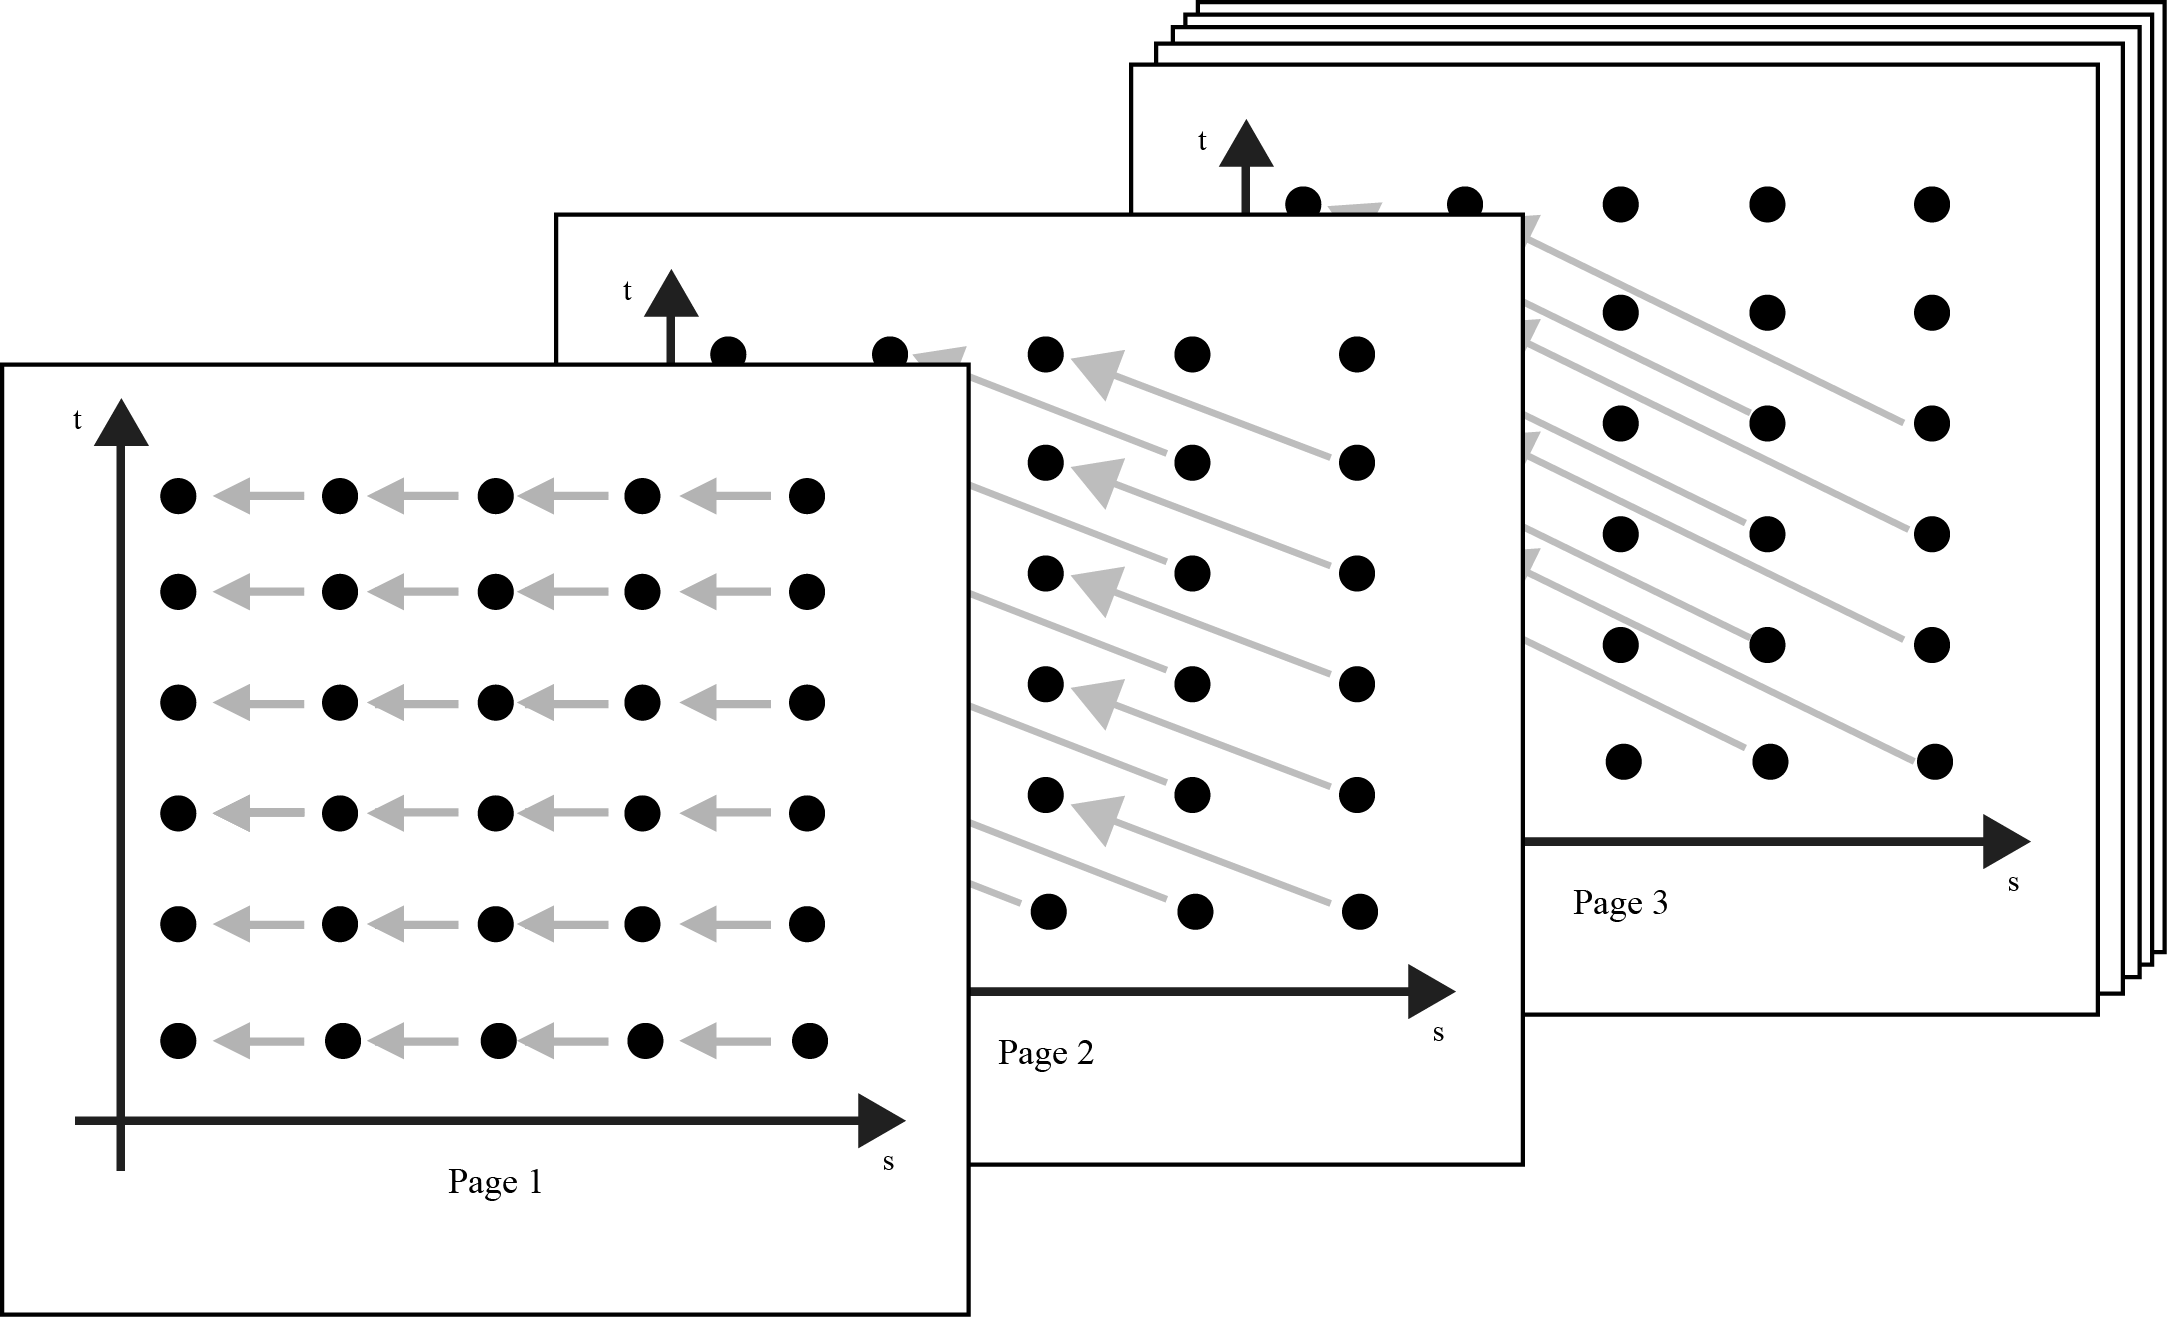
\includegraphics[width=\linewidth,height=0.5\textheight,keepaspectratio]{figures/cover.png}
  \end{center}
       \begin{minipage}{.35\linewidth}
    \begin{flushleft}
      \vspace{2em}
      {\fontsize{6pt}{2pt} \textit{Notes: These are notes live-tex'd
from a graduate course on Étale Cohomology taught by Daniell Litt at the
University of Georgia in Fall 2020. As such, any errors or inaccuracies
are almost certainly my own. } } \\
    \end{flushleft}
    \end{minipage}
    \hfill
    \begin{minipage}{.65\linewidth}
    \end{minipage}
  }







\begin{document}

\date{}
\maketitle
\begin{flushleft}
\textbf{D. Zack Garza} \\
\textit{University of Georgia} \\
\textit{dzackgarza@gmail.com} \\
{\tiny \textit{Last updated:} 2020-10-25 }
\end{flushleft}


\newpage
\tableofcontents

These are notes live-tex'd from a graduate course in Étale Cohomology
taught by Daniel Litt at the University of Georgia in Fall 2020. As
such, any errors or inaccuracies are almost certainly my own.

\medskip
\begin{flushright}
  D. Zack Garza, \today \\
  \currenttime
\end{flushright}

\hypertarget{thursday-august-20}{%
\section{Thursday, August 20}\label{thursday-august-20}}

\begin{quote}
References: \url{https://www.daniellitt.com/tale-cohomology}
\end{quote}

\hypertarget{intro}{%
\subsection{Intro}\label{intro}}

Prerequisites:

\begin{itemize}
\tightlist
\item
  Homological Algebra

  \begin{itemize}
  \tightlist
  \item
    Abelian Categories
  \item
    Derived Functors
  \item
    Spectral Sequences (just exposure!)
  \end{itemize}
\item
  Sheaf theory and sheaf cohomology
\item
  Schemes (Hartshorne II and III)
\end{itemize}

Outline/Goals:

\begin{itemize}
\tightlist
\item
  Basics of etale cohomology

  \begin{itemize}
  \tightlist
  \item
    Etale morphism
  \item
    Grothendieck topologies
  \item
    The etale topology
  \item
    Etale cohomology and the basis theorems
  \item
    Etale cohomology of curves
  \item
    Comparison theorems to singular cohomology
  \item
    Focused on the case where coefficients are a constructible sheaf.
  \end{itemize}
\item
  Prove the Weil Conjectures (more than one proof)

  \begin{itemize}
  \tightlist
  \item
    Proving the Riemann Hypothesis for varieties over finite fields
  \end{itemize}

  \begin{quote}
  One of the greatest pieces of 20th century mathematics!
  \end{quote}
\item
  Topics

  \begin{itemize}
  \tightlist
  \item
    Weil 2 (Strengthening of RH, used in practice)
  \item
    Formality of algebraic varieties (topological features unique to
    varieties)
  \item
    Other things (monodromy, refer to Katz' AWS notes)
  \end{itemize}
\end{itemize}

\hypertarget{what-is-etale-cohomology}{%
\subsection{What is Etale Cohomology?}\label{what-is-etale-cohomology}}

Suppose \(X/\CC\) is a quasiprojective variety: a finite type separated
integral \(\CC\dash\)scheme.

If you take the complex points, it naturally has the structure of a
complex analytic space \(X(\CC)^{\text{an}}\): you can give it the
Euclidean topology, which is much finer than the Zariski topology.

For a nice topological space, we can associate the singular cohomology
\(H^i(X(\CC)^{\text{an}}, \ZZ)\), which satisfies several nice
properties:

\begin{itemize}
\tightlist
\item
  Finitely generated \(\ZZ\dash\)modules
\item
  Extra Hodge structure when tensored up to \(\CC\) (same as \(\CC\)
  coefficients)
\item
  Cycle classes (i.e.~associate to a subvariety a class in cohomology)
\end{itemize}

Goal of etale cohomology: do something similar for much more general
``nice'' schemes. Note that some of these properties are special to
complex varieties

E.g. finitely generated: not true for a random topological space

We'll associate \(X\) a ``nice scheme''
\(\rightsquigarrow H^i(X_{\text{et}}, \ZZ/\ell^n\ZZ)\). Take the inverse
limit over all \(n\) to obtain the \(\ell\dash\)adic cohomology
\(H^i(X_{\text{et}}, \ZZ_\ell)\). You can tensor with \(\QQ\) to get
something with \(\QQ_\ell\) coefficients. And as in singular cohomology,
you can a ``twisted coefficient system''.

What are nice schemes:

\begin{itemize}
\tightlist
\item
  \(X = \spec \OO_k\), the ring of integers over a number field.
\item
  \(X\) a variety over an algebraically closed field

  \begin{itemize}
  \tightlist
  \item
    Typical, most analogous to taking a variety over \(\CC\).
  \end{itemize}
\item
  \(X\) a variety over a non-algebraically closed field
\end{itemize}

Some comparisons between the last two cases:

\begin{itemize}
\tightlist
\item
  For \(\CC\dash\) variety, \(H^i_{\text{sing}}\) will vanish above
  \(i=2d\).
\item
  Over a finite field, \(H^i\) will vanish for \(i>2d+1\) but generally
  not vanish for \(i=2d+1\).
\end{itemize}

In good situations, these are finitely generated
\(\ZZ/\ell^n\ZZ\dash\)modules, have Mayer-Vietoris and excision
sequences, spectral sequences, etc.

Related invariants: for a scheme with a geometric point
\((X, \bar x) \rightsquigarrow \pi_1^{\text{étale}}(X, \bar x)\), which
is a profinite topological group, which is a profinite topological
group.

\begin{quote}
Note: a geometric point is a map from \(\spec X\) to an algebraically
closed field.
\end{quote}

More invariants beyond the scope of this course:

\begin{itemize}
\tightlist
\item
  Higher homotopy groups
\item
  Homotopy type (equivalence class of spaces)
\end{itemize}

So we want homotopy-theoretic invariants for varieties.

\begin{remark}

This cohomology theory is necessarily weird!

\begin{theorem}[Serre]

There does not exists a cohomology theory for schemes over
\(\bar{\FF}_q\) with the following properties:

\begin{enumerate}
\def\labelenumi{\arabic{enumi}.}
\tightlist
\item
  Functorial
\item
  Satisfies the Kunneth formula
\item
  For \(E\) an elliptic curve, \(H^1(E) = \QQ^2\).
\end{enumerate}

\begin{quote}
Slogan: No cohomology theory with \(\QQ\) coefficients.
\end{quote}

\end{theorem}

\begin{proof}

Take \(E\) to be a supersingular elliptic curve. Then
\(\endo(E) \tensor \QQ\) is a quaternion algebra.

Fact: There are no algebra morphisms \(R\to \mat_{2\times 2}(\QQ)\)

\begin{exercise}

Functoriality and Kunneth implies that \(\endo(E)\actson E\) yields an
action on \(H^1(E)\), which is precisely an algebra morphism
\(\endo(E) \to \mat_{2\by 2}(\QQ)\), a contradiction.

\begin{quote}
The content: the sum of two endomorphisms act via their sum on \(H^1\).
\end{quote}

\end{exercise}

\begin{exercise}

Prove the same thing for \(\QQ_p\) coefficients, where \(p\) divides the
characteristic of the ground field.

\begin{quote}
Proof the same, just need to know what quaternion algebras show up.
\end{quote}

\end{exercise}

\end{proof}

\end{remark}

This forces using some funky type of coefficients.

\hypertarget{what-are-the-weil-conjectures}{%
\subsection{What are the Weil
Conjectures?}\label{what-are-the-weil-conjectures}}

Suppose \(X/\FF_q\) is a variety, then
\begin{align*}  
\zeta_X(t) = \exp{\sum_{n>0} { {\abs{X(\FF_{q^n})} \over n} t^n } }
.\end{align*}

Some comments:

\begin{itemize}
\tightlist
\item
  \(\dd{}{t} \log \zeta_X(t)\) is an ordinary generating function for
  the number of rational points.
\item
  Slogan: locations of zeros and poles of a meromorphic function control
  the growth rate of the coefficients of the Taylor series of the
  logarithmic derivative.
\end{itemize}

\begin{exercise}

Make this slogan precise for rational functions, i.e.~ratios of two
polynomials.

\end{exercise}

The conjectures:

\begin{enumerate}
\def\labelenumi{\arabic{enumi}.}
\item
  \(\zeta_x(t)\) is a rational function.
\item
  (Functional equation) For \(X\) smooth and proper
  \begin{align*}  
  \zeta_X(q^{-n} t\inv) = \pm q^{nE \over 2} t^E \zeta_X(t)
  .\end{align*}
\item
  (RH) All roots and poles of \(\zeta_X(t)\) have absolute value
  \(q^{i\over 2}\) with \(i\in \ZZ\), and these are equal to the \(i\)th
  Betti numbers if \(X\) lifts to characteristic zero.
\end{enumerate}

\begin{quote}
Note: we'll generalize betti numbers so this makes sense in general.
\end{quote}

All theorems! Proofs:

\begin{enumerate}
\def\labelenumi{\arabic{enumi}.}
\item
  Dwork, using \(p\dash\)adic methods. Proof here will follow from the
  fact that \(H^i_{\text{étale} }\) are finite-dimensional. Related to
  Lefschetz Trace Formula (how Grothendieck thought about it).
\item
  Grothendieck, follows from some version of Poincaré duality.
\item
  (and 4) Deligne.
\end{enumerate}

\hypertarget{euler-product}{%
\subsubsection{Euler Product}\label{euler-product}}

Let \(\abs X\) denote the closed points of \(X\), then there is an Euler
product:
\begin{align*}  
\zeta_X(q^{-n} t\inv) = \pm q^{nE \over 2} t^E \zeta_X(t)
&= \prod_{x\in \abs{X}} \exp{t^{\deg (x)} + {t^{2\deg (x)} \over 2} + \cdots} \\
&= \prod_{x\in \abs X} \exp{-\log(1-t^{\deg(x)})} \\
&= \prod_{x\in \abs X} {1 \over 1 - t^{\deg(x)}}
.\end{align*}

\begin{exercise}

Check the first equality. If you have a point of \(\deg(x) = n\), how
many \(\FF_{q^n}\) points does this contribute? I.e., how many maps are
there \(\spec(\FF_{q^n}) \to \spec(\FF_{q^n})\) over \(\FF_q\)?

There are exactly \(n\): it's \(\gal(\FF_{q^n} / \FF_q)\). But then
division by \(n\) drops this contribution to one.

\end{exercise}

We can keep going by expanding and multiplying out the product:
\begin{align*}  
\prod_{x\in \abs X} {1 \over 1 - t^{\deg(x)}}
&= \prod_{x\in \abs X} (1 + t^{\deg(x)} + t^{2 \deg(x)}) \\
&= \sum_{n\geq 0} \qty{\text{\# of Galois-stable subset of $X(\bar \FF_{q^n})$ of size $n$}}t^n
.\end{align*}

Why? If you have a degree \(x\) point, it contributes a stable subset of
size \(x\): namely the \(\FF_{q^n}\) points of \(\FF_{q^n}\). Taking
Galois orbits like that correspond to multiplying this product.

But these are the points of some algebraic variety:
\begin{align*}  
\cdots 
= \sum_{n\geq 0} \abs{\sym^n(X)(\FF_q)} t^n
,\end{align*} where \(\sym^n(X) \da X^n/\Sigma_n\), the action of the
symmetric group. Why is that? A \(\bar \FF_q\) point of \(\sym^n(X)\) is
an unordered \(n\dash\)tuple of \(\bar \FF_q\) points without an
ordering, and asking them to be Galois stable is the same as saying that
they are an \(\FF_q\) point.

\begin{theorem}[First Weil Conjecture for Curves]

For \(X\) a smooth proper curve over \(\FF_q\), \(\zeta_X(t)\) is
rational.

\end{theorem}

\begin{proof}

Claim: there is a set map
\begin{align*}  
\sym^n X &\to \pic^n X \\
D &\mapsto \OO(D)
.\end{align*}

\begin{quote}
Here the divisor is an \(n\dash\)tuple of points.
\end{quote}

What are the fibers over a line bundle \(\OO(D)\)? A linear system,
i.e.~the projectivization of global sections \(\PP \Gamma(X, \OO(D))\).
What is the expected dimension? To compute the dimension of the space of
line bundles on a curve, use Riemann-Roch:
\begin{align*}  
\dim \PP\Gamma(X, \OO(D)) = \deg(D) + 1 - g + \dim H^1(X, \OO(D)) - 1
.\end{align*} where the last \(-1\) comes from the fact that this is a
projective space.

Claim: if \(\deg(D) = 2g-2\), then \(H^1(X, \OO(D)) = 0\).

This is because it's dual to \(H^0(X, \OO(K-D))\dual\), but this has
negative degree and a line bundle of negative degree can never have
sections.

\begin{quote}
Note: should check to make sure you know why this is true!
\end{quote}

Thus the fibers are isomorphic to \(\PP^{n-g}\) for \(n>2g-2\). Now make
a reduction (exercise: justify why):

Wlog assume \(X(\FF_q) \neq \emptyset\). In this case,
\(\pic^n(X) \cong \pic^{n+1}(X)\) for all \(n\), since you can take
\(\OO(P)\) for \(P\) a point, a degree 1 line bundle, and tensor with
it. It's an isomorphism because you can tensor with the dual bundle to
go back.

Thus for all \(n>2g-2\),
\begin{align*}  
\abs{\sym^n(X)(\FF_q)} 
= \abs{\PP^{n-g}(\FF_q)} \cdot \abs{\pic^n(X)(\FF_q)}
= \abs{\PP^{n-g}(\FF_q)} \cdot \abs{\pic^0(X)(\FF_q)}
.\end{align*}

Thus \(\zeta_X(t)\) is a polynomial plus
\(\sum_{n>2g-2} \abs{\pic^n(X)(\FF_q)}\qty{1+q+q^2+\cdots+q^{n-g}}t^n\).

\begin{exercise}

Show that this is a rational function using the formula for a geometric
series.

\end{exercise}

\end{proof}

\begin{theorem}[Functional Equation]

The functional equation in the case of curves:
\begin{align*}  
\zeta_X(q^{-1} t^{-1} ) = \pm q^{2-2g \over 2} t^{2-2g} \zeta_X(t)
.\end{align*}

\end{theorem}

\begin{exercise}[Important]

Where it comes from in terms of \(\sym^n\): Serre duality.

\end{exercise}

We'll show the RH later.

\begin{theorem}[Dwork]

Suppose \(X/\FF_q\) is any variety, then \(\zeta_X(t)\) is rational
function.

\end{theorem}

\begin{quote}
Roughly known to Weil, hinted at in original paper
\end{quote}

\begin{proof}[Grothendieck]

Idea: take Frobenius (intentionally vague, arithmetic vs geometric vs
\ldots) \(F:X\to X\), then \(X(\FF_q)\) are the fixed points of \(F\)
acting on \(X_{\bar \FF_q}\), and the \(\FF_{q^n}\) points are the fixed
points of \(F^n\).

Uses the Lefschetz fixed point formula, which will say for
\(\ell\neq \ch(\FF_q)\),
\begin{align*}  
\abs{X(\FF_{q^n})} = \sum_{i=0}^{2\dim(X)} (-1)^i \tr(F^n) H^i_c(X_{\FF_q}, \QQ_\ell)
.\end{align*}

\begin{quote}
Here \(H^i_c\) is compactly supported cohomology, we'll define this
later in the course.
\end{quote}

\begin{lemma}

\begin{align*}  
\exp{\sum {\tr(F^n) \over n}t^n  }\quad\text{is rational}
.\end{align*}

\end{lemma}

This lemma implies the result, because if you plug the trace formula
into the zeta function, you'll get an alternating product
\(f \cdots {1\over g} \cdot h \cdot {1\over j} \cdots\) of functions of
the form in the lemma, which is still rational.

\begin{proof}[Of Lemma]

It suffices to treat the case \(\dim(V) = 1\), because otherwise you can
just write this as a sum of powers of eigenvalues.

Then you have a scalar matrix, so you obtain
\begin{align*}  
\exp{ \sum {\alpha^n \over n} t^n} = \exp{ -\log(1 - \alpha t)} = {1 \over 1-\alpha t}
,\end{align*} which is rational.

\end{proof}

\end{proof}

This proves rationality, contingent on

\begin{enumerate}
\def\labelenumi{\arabic{enumi}.}
\tightlist
\item
  The Lefschetz fixed point formula
\item
  The finite dimensionality of etale cohomology
\end{enumerate}

\begin{exercise}

Try to figure out how Poincaré duality should give the functional
equation.

\begin{quote}
Hint: try the lemma on a vector space where \(F\) scales a bilinear
form.
\end{quote}

\end{exercise}

\begin{theorem}[Serre, Kahler Analog]

Suppose \(X/\CC\) is a smooth projective variety and
\([H] \in H^2(X(\CC), \CC)\) is a hyperplane class (corresponds to
intersection of generic hyperplane or the first Chern class of an ample
line bundle).

Suppose \(F:X\to X\) is an endomorphism such that \(f^*[H] = q[H]\) for
some \(q\in \ZZ_{\geq 1}\).

Define
\begin{align*}  
L(F^n) \definedas 
\sum_{i=0}^{2\dim(X)} (-1)^i \tr\qty{ F^n \st H^i(X_{\FF_q}, \QQ_\ell)}
.\end{align*} and
\begin{align*}  
\zeta_{X, F}(t) \da
\exp{\sum_{n=1}^\infty {L(F^n) \over n}t^n }
.\end{align*}

Then \(\zeta_{X, F}(t)\) satisfies the RH: the zeros and poles are of
absolute value \(q^{i\over 2}\). Equivalently, the eigenvalues
\(\lambda\) of \(F^n\) actings on \(H^i(X, \CC)\) all satisfy
\(\abs{\lambda} = q^{i\over 2}\).

\end{theorem}

Next time, to review

\begin{itemize}
\tightlist
\item
  Étale morphisms
\item
  Definition of a site
\end{itemize}

\newpage

\newpage
\section{Indices}
\listoftodos[List of Todos]

% Hook into amsthm environments to list them.
\renewcommand{\listtheoremname}{Definitions}
\listoftheorems[ignoreall,show={definition}, numwidth=3.5em]

\renewcommand{\listtheoremname}{Theorems}
\listoftheorems[ignoreall,show={theorem,proposition}, numwidth=3.5em]

\renewcommand{\listtheoremname}{Exercises}
\listoftheorems[ignoreall,show={exercise}, numwidth=3.5em]

\listoffigures


\printbibliography[title=Bibliography]


\end{document}
